\documentclass[10pt,a4paper]{article}
\usepackage[utf8]{inputenc}
\usepackage{amsmath}
\usepackage{amsfonts}
\usepackage{amssymb}
\usepackage{graphicx}
\usepackage{float}
\begin{document}
\begin{center}
Results analysis for homework 1\\
Marat Khabibullin
\end{center}

Let's look at the program output shown in Figure 1. One can see (according to p-values) there is a depedency between Sales volume and predictors under consideration and Newspaper predictor is the least significant (because of the high p-value).\\
Considering mean RSS, we have higher value for the test set and it could be explained by the fact that the model has been created using training data and best fits for this data set.\\
\\
Scatterplots are shown in Figure 2 and 3 and one can notice clear linear dependance.

\begin{figure}[H]
\centering
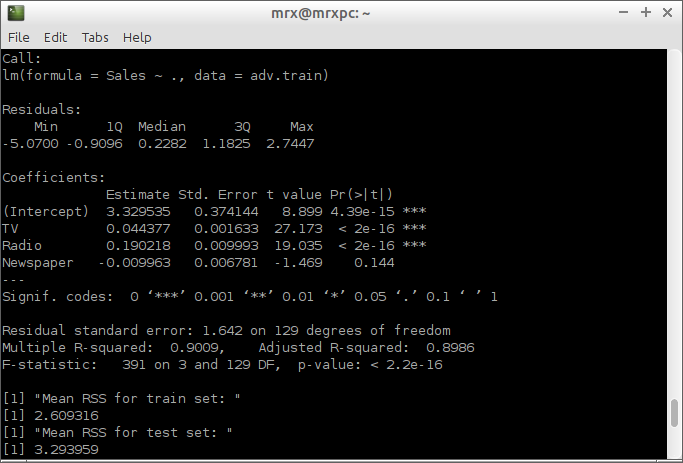
\includegraphics[width=140mm]{figures/ord.png}
\caption{Model with all predictors \label{overflow}}
\end{figure}

\begin{figure}[H]
\centering
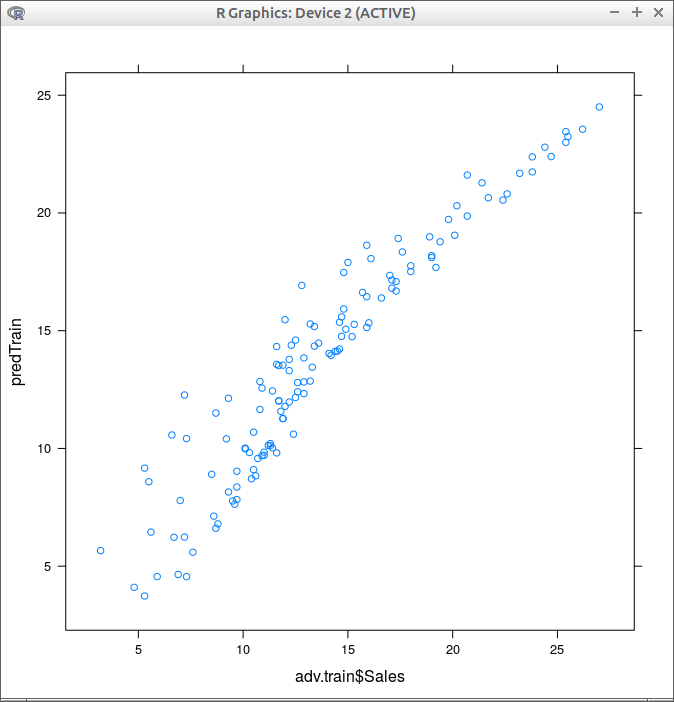
\includegraphics[width=140mm]{figures/pltOrdTrain.png}
\caption{Scatterplot for training set (all predictors) \label{overflow}}
\end{figure}

\begin{figure}[H]
\centering
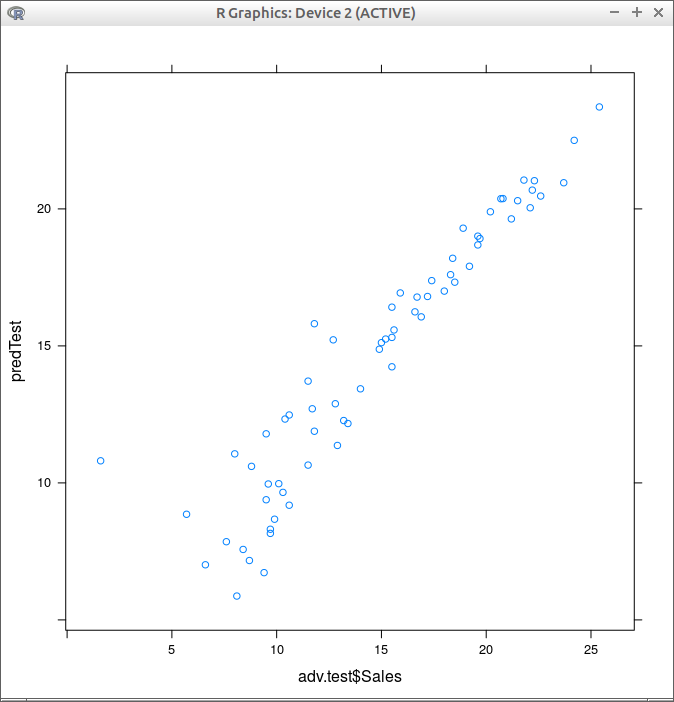
\includegraphics[width=140mm]{figures/pltOrdTest.png}
\caption{Scatterplot for test set (all predictors) \label{overflow}}
\end{figure}
\vspace{5cm}

Now let's consider program output for model with Newspapers predictor removed (Fig. 4). One may notice in comparison with the previous reults (see Fig. 1) F-statistics value has grown significantly, so we can conclude model has become better (better discribes real data).\\
Moreover, rss values are almost the same as in the model with all predictors. It proves the Nespaper predictor's insignificance.\\
Scatterplots in Figures 5 and 6 still show linear behaviour.\\

\begin{figure}[H]
\centering
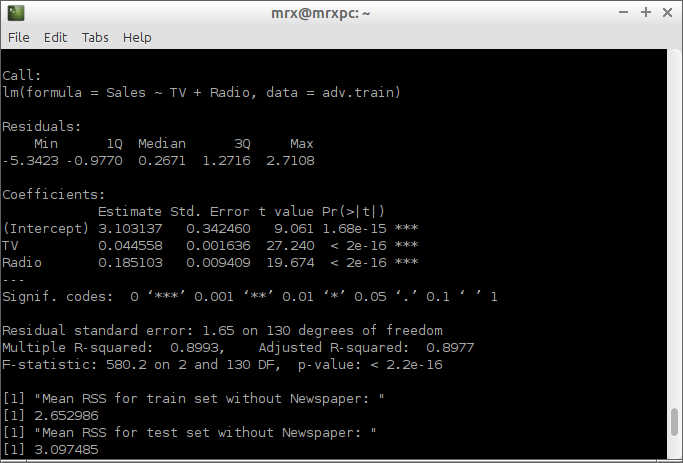
\includegraphics[width=140mm]{figures/noNews.png}
\caption{Model with Newspapers predictor removed \label{overflow}}
\end{figure}

\begin{figure}[H]
\centering
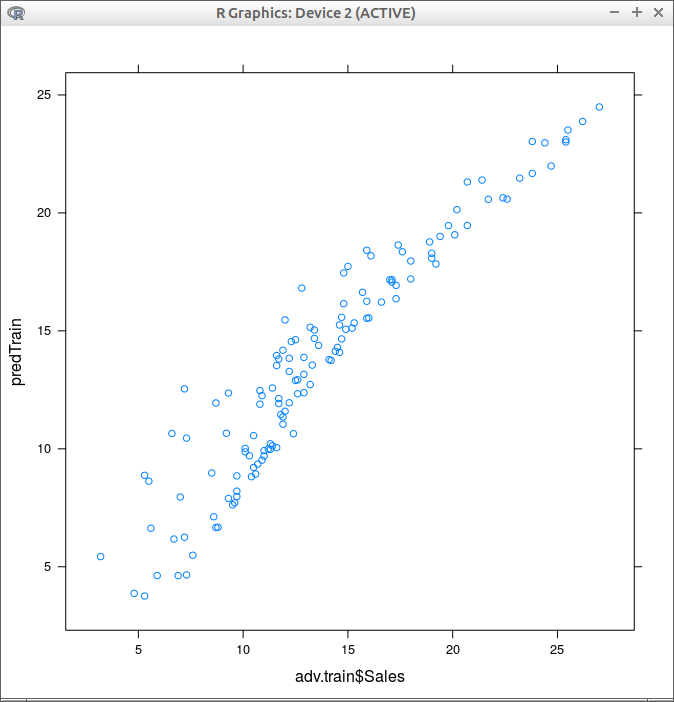
\includegraphics[width=140mm]{figures/pltNoNewsTrain.png}
\caption{Scatterplot for training set (Newspapers predictor removed) \label{overflow}}
\end{figure}

\begin{figure}[H]
\centering
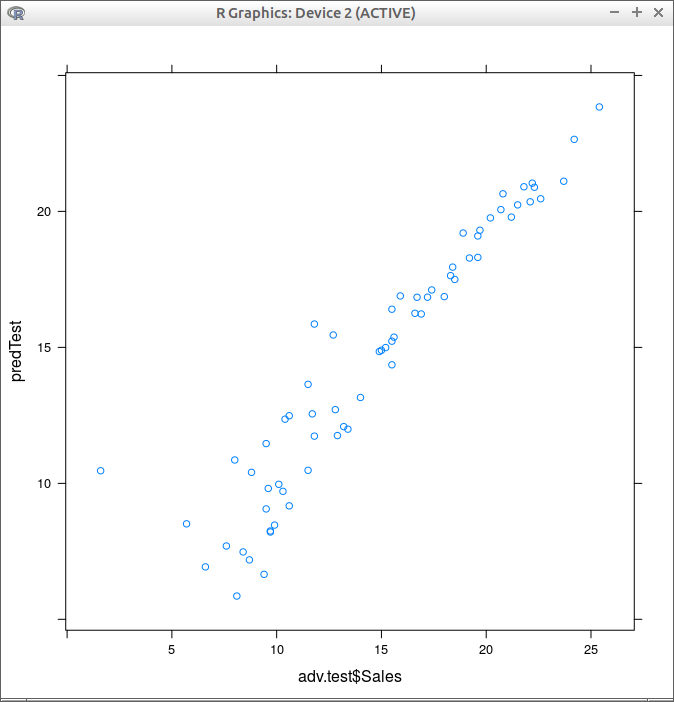
\includegraphics[width=140mm]{figures/pltNoNewsTest.png}
\caption{Scatterplot for test set (Newspapers predictor removed) \label{overflow}}
\end{figure}
\vspace{5cm}

Next program output (Fig. 7) shows the model with TV predictor removed. F-statistic value has become very low that is corresponds to the fact the TV predictor is significant in our model in general. Moreover, removing significant predictor we have increased rss values for both training and test data sets.\\
Scatterplots in Figures 8 and 9 also reflect the fact of removing significant predictor - the dependencies are not linear anymore, predicted data badly corressponts to actual one.

\begin{figure}[H]
\centering
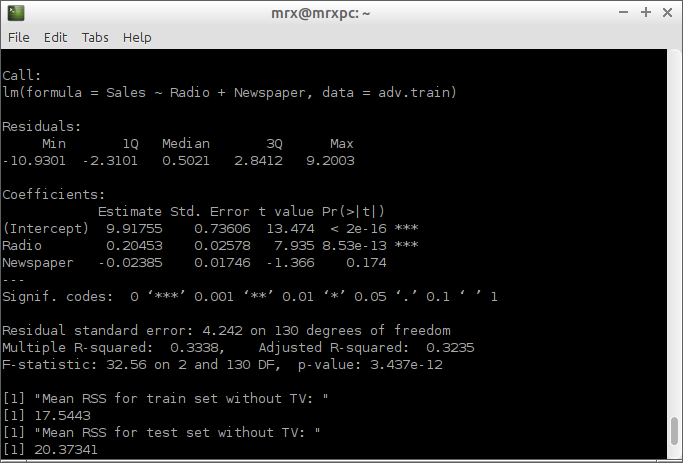
\includegraphics[width=140mm]{figures/noTv.png}
\caption{Model with Tv predictor removed \label{overflow}}
\end{figure}

\begin{figure}[H]
\centering
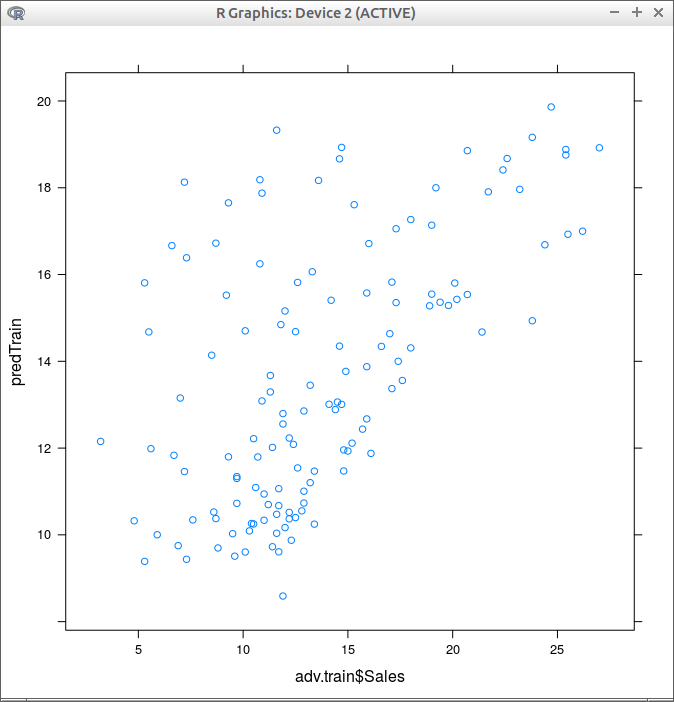
\includegraphics[width=140mm]{figures/pltNoTvTrain.png}
\caption{Scatterplot for training set (Tv predictor removed) \label{overflow}}
\end{figure}

\begin{figure}[H]
\centering
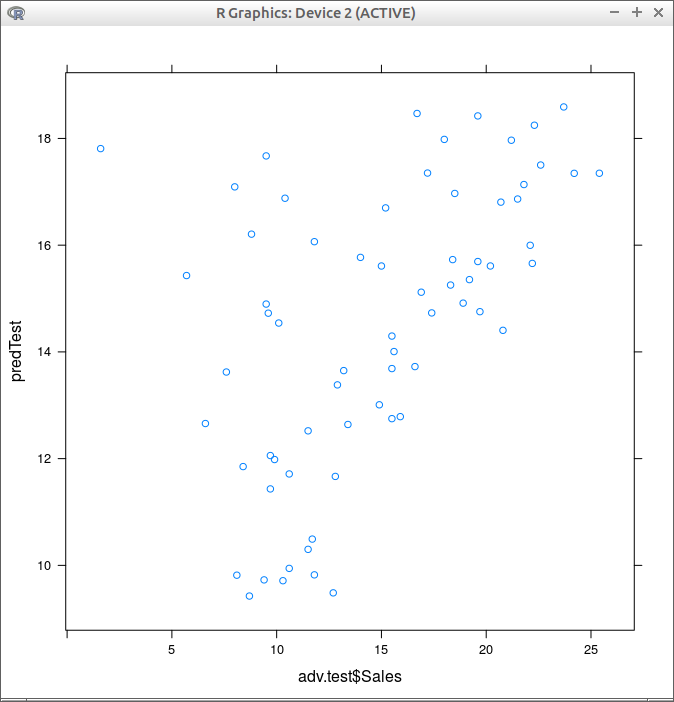
\includegraphics[width=140mm]{figures/pltNoTvTest.png}
\caption{Scatterplot for test set (Tv predictor removed) \label{overflow}}
\end{figure}
\vspace{5cm}

The last model to consider is one with all predictor removed (Fig. 10). As we can see rss values have drastically increased in comparison with the initial model values. Also, scatterplots in Figures 11 and 12 show predicted Sales volumes are constant and equals to calculated Intercept value (see Fig. 10). It clearly represents independency of model predictions and input data making such model useless.

\begin{figure}[H]
\centering
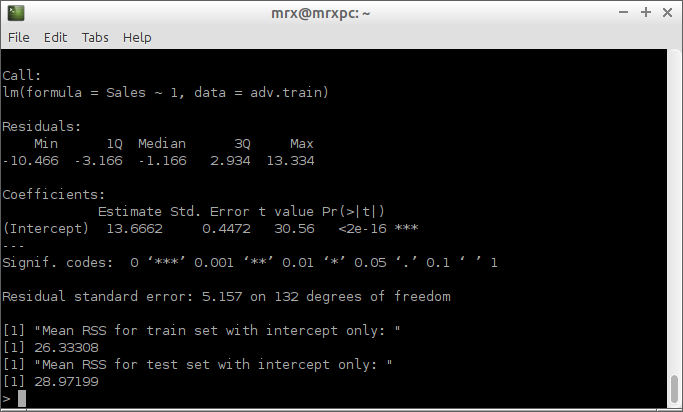
\includegraphics[width=140mm]{figures/int.png}
\caption{Model with all predictors removed \label{overflow}}
\end{figure}

\begin{figure}[H]
\centering
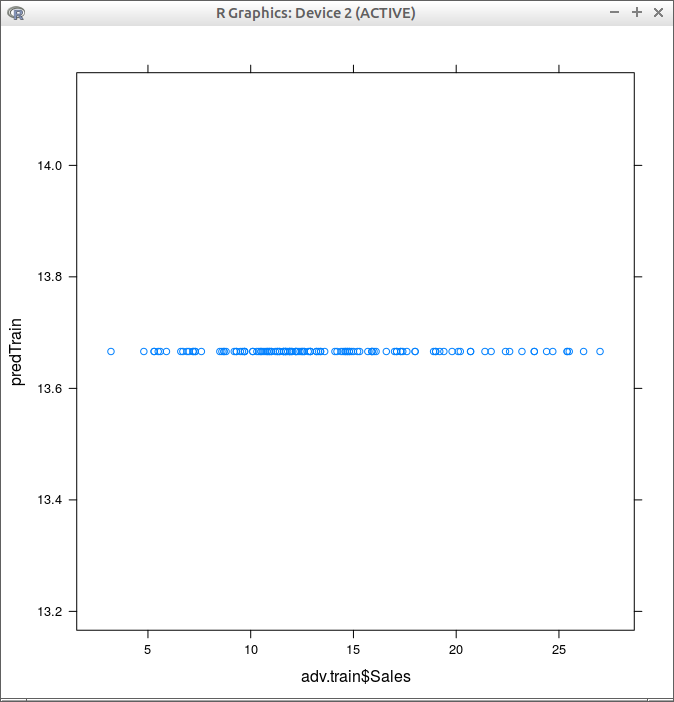
\includegraphics[width=140mm]{figures/pltIntTrain.png}
\caption{Scatterplot for training set (all predictors removed) \label{overflow}}
\end{figure}

\begin{figure}[H]
\centering
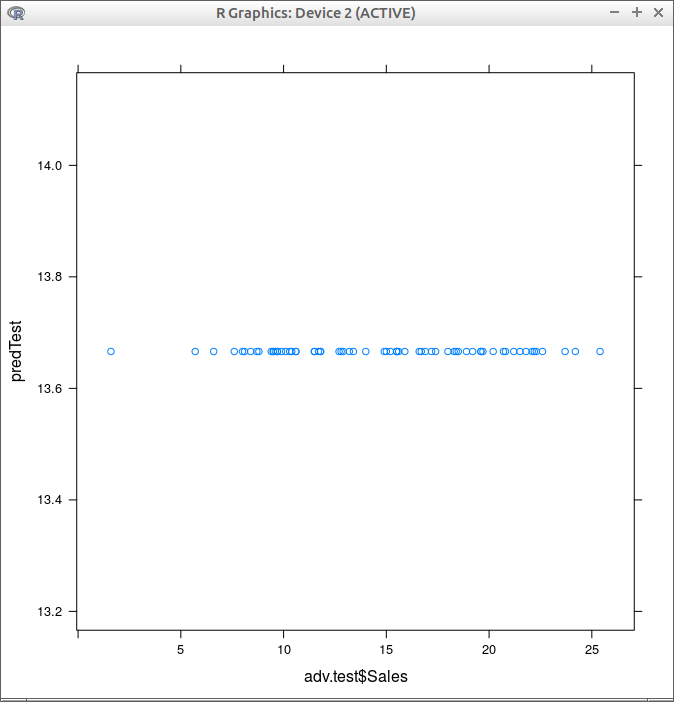
\includegraphics[width=140mm]{figures/pltIntTest.png}
\caption{Scatterplot for test set (all predictors removed) \label{overflow}}
\end{figure}

In conclusion it is important to note that on different program runs different result are observed. For example, one program run can give higher rss value for test data set in comparison to training data set. This fact could be explained by randomness of choosing what part of all the input data will be the test one and what will be the training one.\\

\vspace{5cm}

\begin{center}
Additional task: polynomial regression
\end{center}
Let's look at the Figures 13, 14, 15 and 16 representing polynomial regression models with degrees 1, 2, 3 and 4 respectively.\\
First of all, F-statistics are significantly lower in comparison with one in linear model with Newspapers predictor removed (of course, current and previous results are obtained from different program runs, but still avarage value of F-statistics for linear model with Newspapers predictor removed between runs is close to 500). Moreovere, as the degree is increasing the F-statistics value is decreasing. Also, while degree is increasing predictors become more and more insignificant having predictor in the power of 1 the most significant among the others.\\
To study models' suitability AIC and BIC values are also shown. As one can notice, both grow slowly as polynomial degree increases having average value approximately equals to 700. It is important to note AIC and BIC values for linear model with Newspapers predictor removed are approximately 530.\\
Mean RSS values for training and test data are pretty high and remain almost unchanged as polynomial degree increases.\\
Figures 17 - 20 and 21 - 24 show scatterplots for training and test data respectively. As degree is increasing the scatterplots are almost unchanged and resemble scatterblot for degree = 1. It prooves the fact predictors in powers higher than 1 are least significant and don't affect the model much.\\
\\
All the obtained results show the polynomial models are less suitable for the data set under study then linear ones and the higher the degree the worst model describes our data. So, speaking about using polynomial regression for this task the best choice is 2nd degree polynomial.


\begin{figure}[H]
\centering
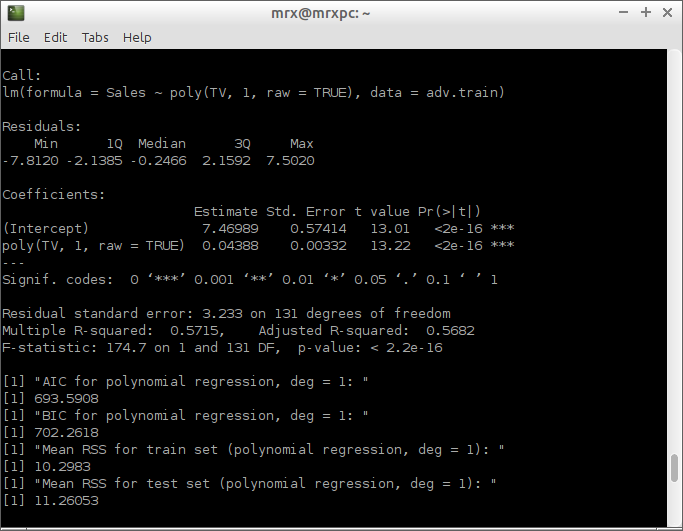
\includegraphics[width=140mm]{figures2/poly1.png}
\caption{Polynomial regression with deg = 1 \label{overflow}}
\end{figure}

\begin{figure}[H]
\centering
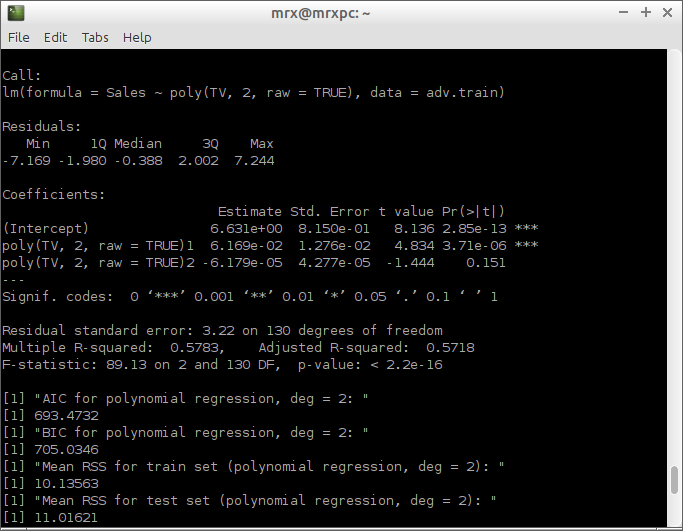
\includegraphics[width=140mm]{figures2/poly2.png}
\caption{Polynomial regression with deg = 2 \label{overflow}}
\end{figure}

\begin{figure}[H]
\centering
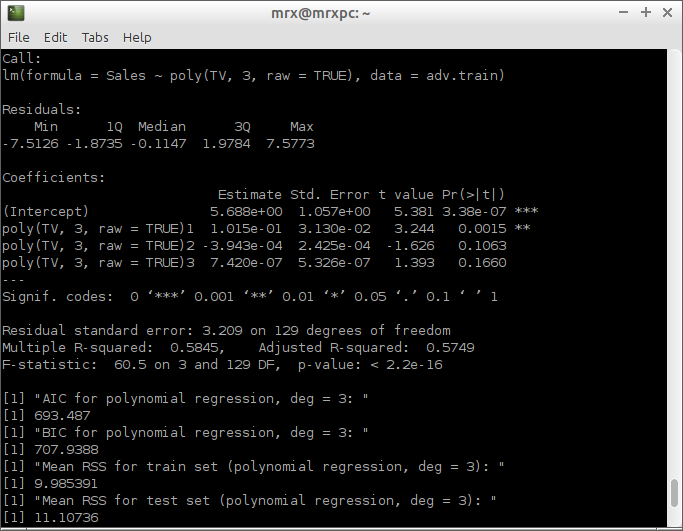
\includegraphics[width=140mm]{figures2/poly3.png}
\caption{Polynomial regression with deg = 3 \label{overflow}}
\end{figure}

\begin{figure}[H]
\centering
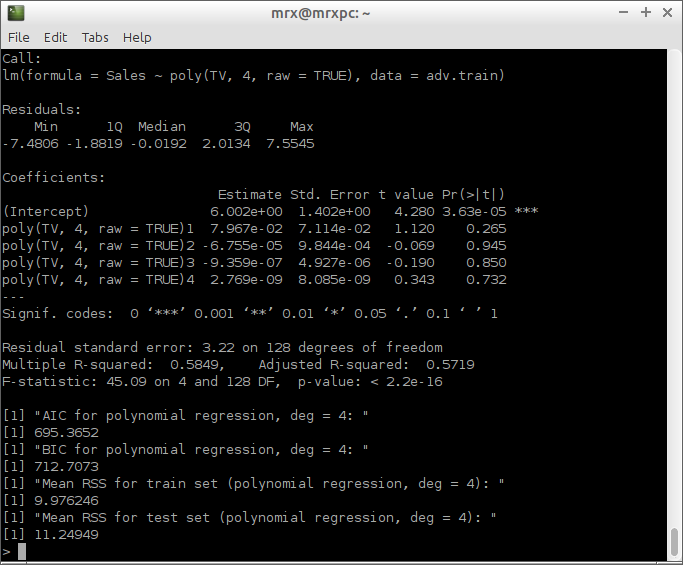
\includegraphics[width=140mm]{figures2/poly4.png}
\caption{Polynomial regression with deg = 4 \label{overflow}}
\end{figure}

\begin{figure}[H]
\centering
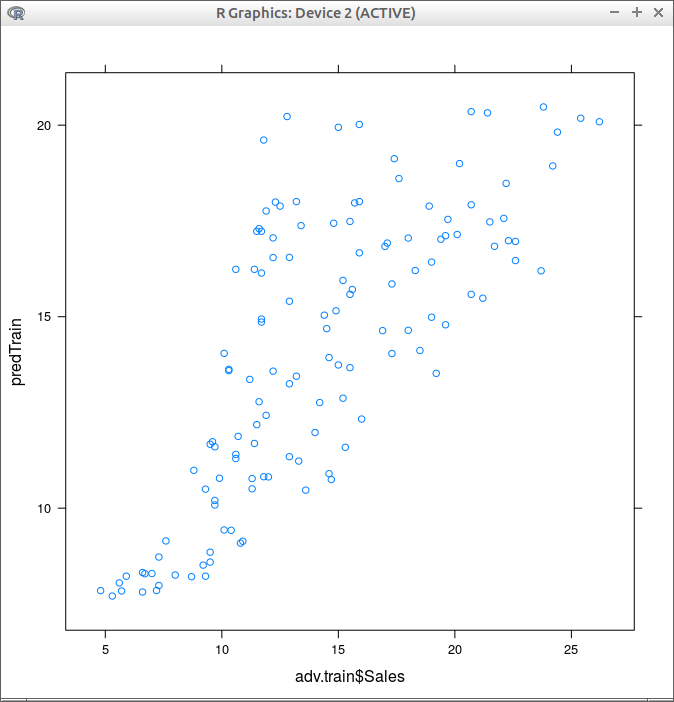
\includegraphics[width=140mm]{figures2/pltTr1.png}
\caption{Scatterplot for training set (polynomial regression with deg = 1) \label{overflow}}
\end{figure}

\begin{figure}[H]
\centering
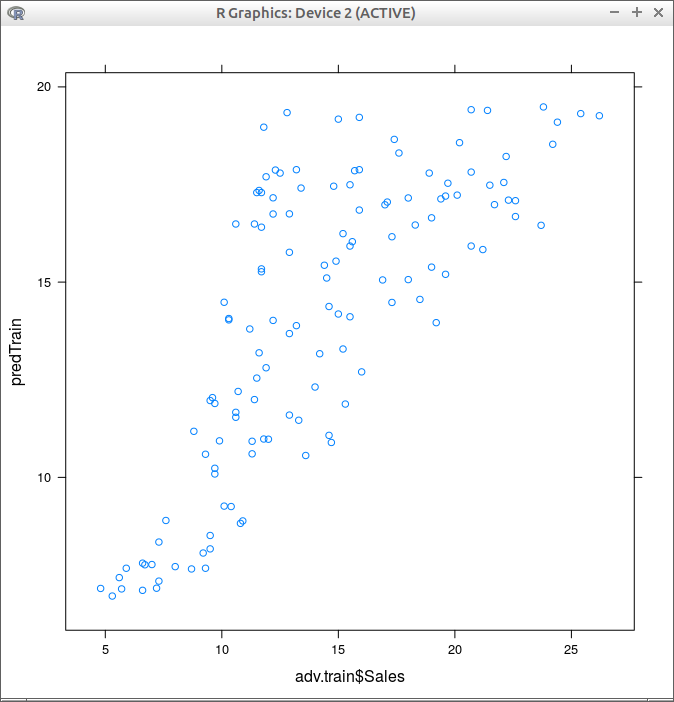
\includegraphics[width=140mm]{figures2/pltTr2.png}
\caption{Scatterplot for training set (polynomial regression with deg = 2) \label{overflow}}
\end{figure}

\begin{figure}[H]
\centering
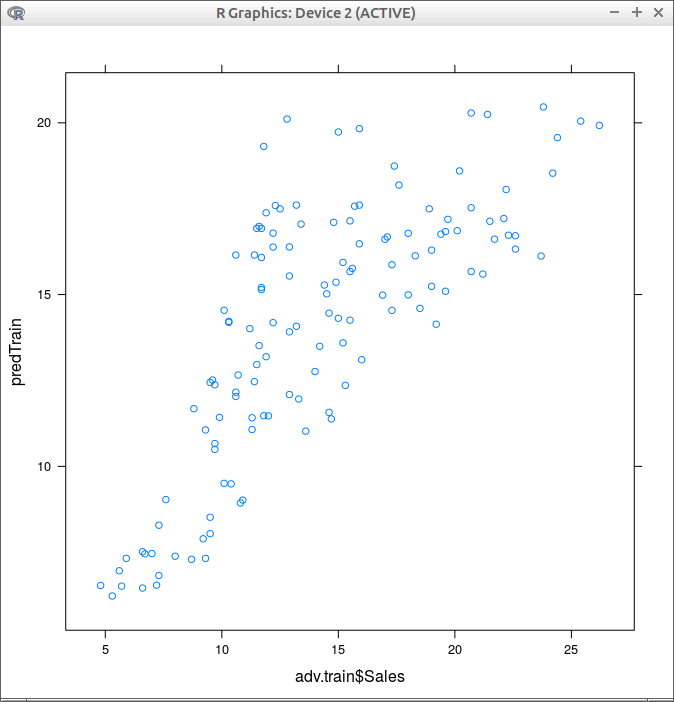
\includegraphics[width=140mm]{figures2/pltTr3.png}
\caption{Scatterplot for training set (polynomial regression with deg = 3) \label{overflow}}
\end{figure}

\begin{figure}[H]
\centering
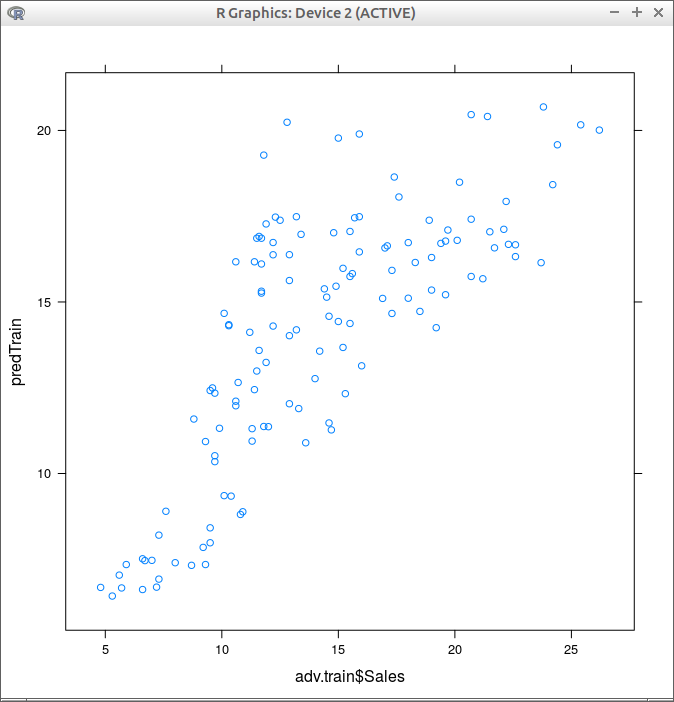
\includegraphics[width=140mm]{figures2/pltTr4.png}
\caption{Scatterplot for training set (polynomial regression with deg = 4) \label{overflow}}
\end{figure}

\begin{figure}[H]
\centering
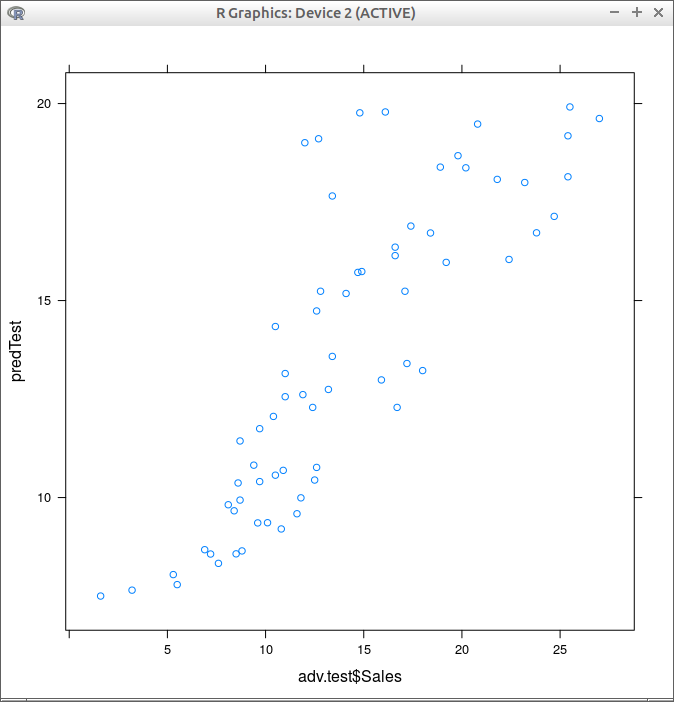
\includegraphics[width=140mm]{figures2/pltTe1.png}
\caption{Scatterplot for test set (polynomial regression with deg = 1) \label{overflow}}
\end{figure}

\begin{figure}[H]
\centering
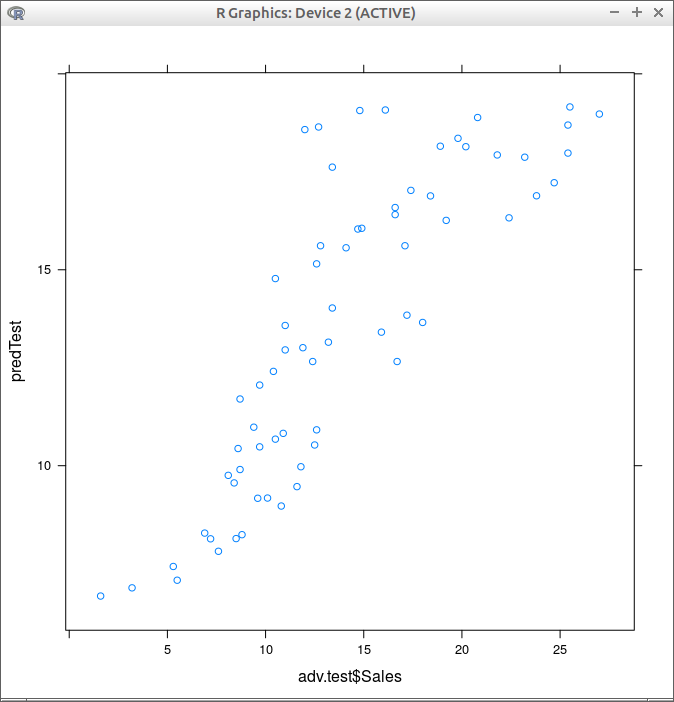
\includegraphics[width=140mm]{figures2/pltTe2.png}
\caption{Scatterplot for test set (polynomial regression with deg = 2) \label{overflow}}
\end{figure}

\begin{figure}[H]
\centering
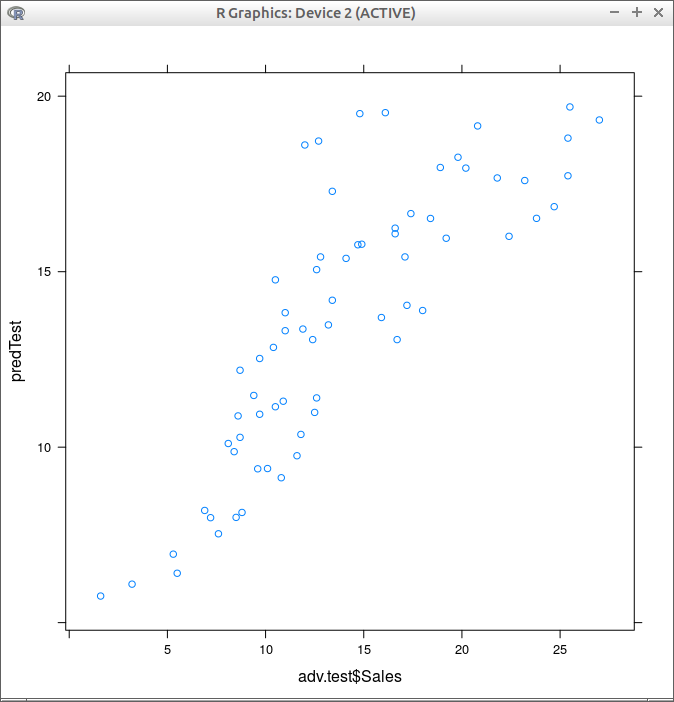
\includegraphics[width=140mm]{figures2/pltTe3.png}
\caption{Scatterplot for test set (polynomial regression with deg = 3) \label{overflow}}
\end{figure}

\begin{figure}[H]
\centering
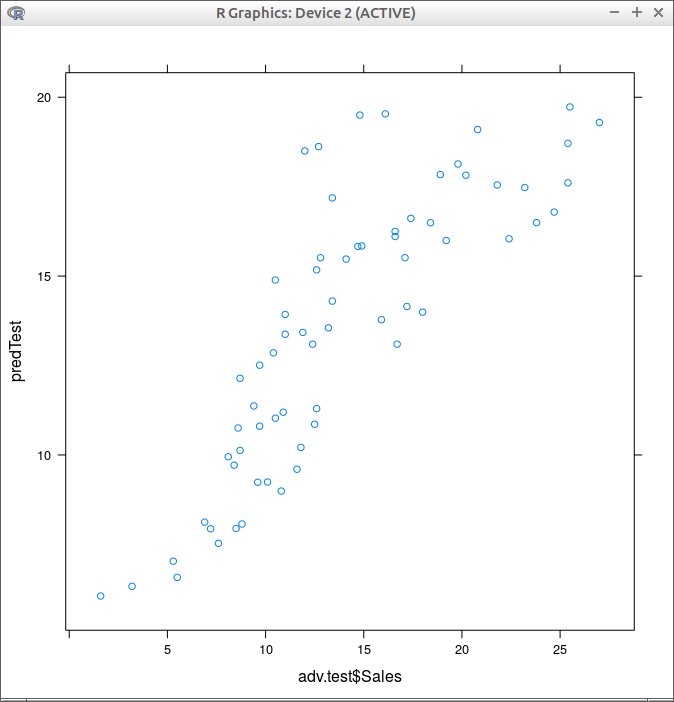
\includegraphics[width=140mm]{figures2/pltTe4.png}
\caption{Scatterplot for test set (polynomial regression with deg = 4) \label{overflow}}
\end{figure}

\end{document}